%! TeX program = lualatex
%! TeX root = main.tex

\def\basedir{/home/theammir/labs/asd/lab2.6/res}
\input{/home/theammir/labs/asd/template/template.tex}

\usepackage{graphicx}
\usepackage[hypcap=false]{caption}
\usepackage{framed}
\usepackage{amsmath}

\begin{document}
\thetitlepage{6}{ІМ-42}{Туров Андрій Володимирович}{28}
\def\thelabid{lab2.6}

\taskdesc%
\begin{enumerate}
  \item Представити напрямлений та ненапрямлений графи iз заданими параметрами так само, як у лабораторнiй роботi №3.\par
    \emph{Вiдмiннiсть 1:} коефiцiєнт $k = 1.0 - n_3 * 0.01 - n_4 * 0.005 - 0.05$.\par
    \emph{Відмінність 2:} матриця ваг $W$ формується таким чином:
    \begin{enumerate}
      \item матриця B розмiром $n*n$ заповнюється згенерованими випадковими числами в дiапазонi $[0, 2.0)$;
      \item одержується матриця $C$:
        \begin{align*}
          c_{ij} = \text{ceil} (b_{ij} * 100 * a_{undir_{ij}}),& \\
          \quad c_{ij} \in C,\, b_{ij} \in B,\, a_{undir_{ij}} \in A_{undir}
        \end{align*}
      \item одержується матриця $D$, у якiй
        \begin{align*}
          d_{ij} = 0,\, \text{якщо}\ c_{ij} = 0,& \\
          d_{ij} = 1,\, \text{якщо}\ c_{ij} > 0;& \\
          \quad d_{ij} \in D, c_{ij} \in C;
        \end{align*}
      \item одержується матриця $H$, у якiй
        \begin{align*}
          h_{ij} = 1,\, \text{якщо}\ d_{ij} \ne d_{ji},\,\\
          \text{та}\ h_{ij} = 0\ \text{в iншому випадку};\;
        \end{align*}
      \item $\text{Tr}$ --- верхня трикутна матриця з одиниць $(tr_{ij} = 1\ \text{при}\ i < j)$;
      \item матриця ваг $W$ симетрична, i її елементи одержуються за формулою:
        $w_{ij} = w_{ji} = \left(d_{ij} + h_{ij} * tr_{ij}\right) * c_{ij}$.
    \end{enumerate}
  \item Створити програму для знаходження мiнiмального кiстяка за алгоритмом Краскала при $n_4$ — парному i за алгоритмом Прiма — при непарному.
    При цьому у програмi:
    \begin{itemize}
      \item графи представляти у виглядi динамiчних спискiв, обхiд графа, додавання, вiднiмання вершин, ребер виконувати як функцiї з вершинами вiдповiдних спискiв;
      \item у програмі виконання обходу відображати покроково, черговий крок виконувати за натисканням кнопки у вікні або на клавіатурі.
    \end{itemize}
  \item Пiд час обходу графа побудувати дерево його кiстяка. У програмi дерево кiстяка виводити покроково у процесi виконання алгоритму.
\end{enumerate}

\taskspec%
$\overline{n_1 n_2 n_3 n_4} = 4228$;\\
Кількість вершин --- $10 + n_3 = 12$.\\
Розміщення вершин --- прямокутником з вершиною в центрі.\\
Знаходження мінімального кістяка за допомогою алгоритма Краскала.

\codetext{rust}

\section{Вивід програми}

\begin{minipage}[t]{0.7\linewidth}
  \begin{center}
    \begin{framed}
      \noindent%
      Матриця ваг:\\
        {\ttfamily\obeyspaces\obeylines\footnotesize%
 \  0 166 197 148 inf inf 162 inf inf inf 171 inf
  166   0 inf 179 inf inf inf 150 inf 136 153 188
  197 inf   0 inf inf 180 154 141 inf 132 138 inf
  148 179 inf   0 inf 198 inf 199 164 162 inf 167
  inf inf inf inf   0 143 190 inf inf inf 187 inf
  inf inf 180 198 143   0 inf 182 inf 157 inf inf
  162 inf 154 inf 190 inf   0 inf inf inf 176 inf
  inf 150 141 199 inf 182 inf   0 inf 153 inf inf
  inf inf inf 164 inf inf inf inf   0 inf 187 148
  inf 136 132 162 inf 157 inf 153 inf   0 inf inf
  171 153 138 inf 187 inf 176 inf 187 inf   0 159
  inf 188 inf 167 inf inf inf inf 148 inf 159   0
        }
    \end{framed}
  \end{center}
\end{minipage}
\hfill
\vspace{1em}

Сума ваг мінімального кістяка --- 1618.

\section{Зображення}

\begin{figure}[ht!]
  \center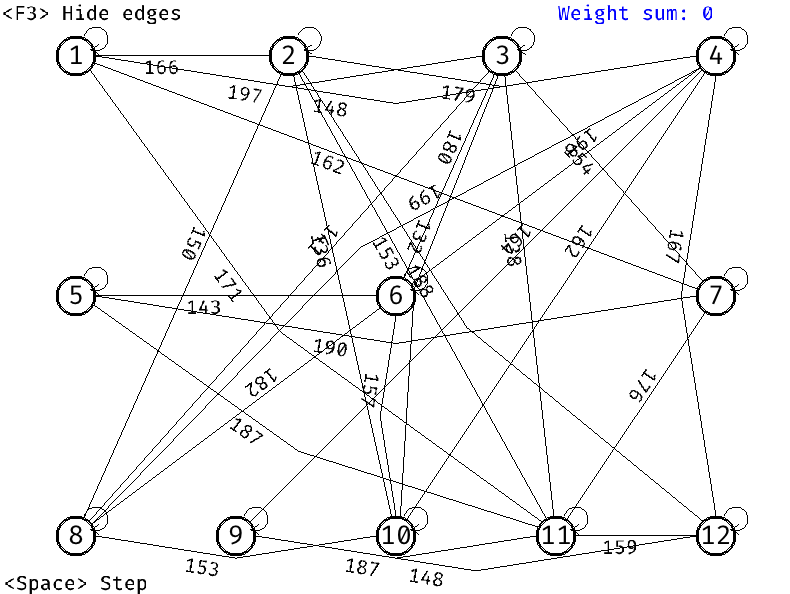
\includegraphics[width=0.5\linewidth]{graph.png}
  \caption{Граф на початку програми}
\end{figure}
\begin{figure}[ht!]
  \center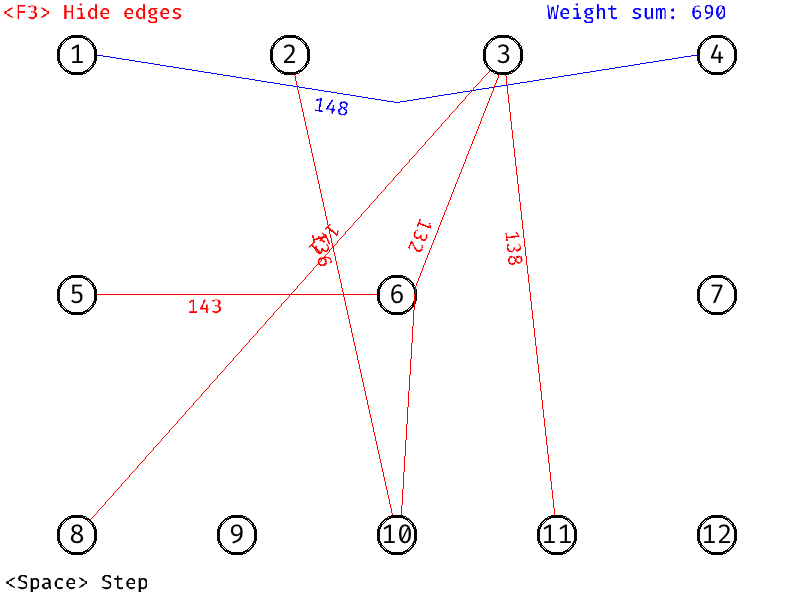
\includegraphics[width=0.5\linewidth]{in_progress.png}
  \caption{Граф під час побудови кістяка (ребра приховані)}
\end{figure}
\begin{figure}[ht!]
  \center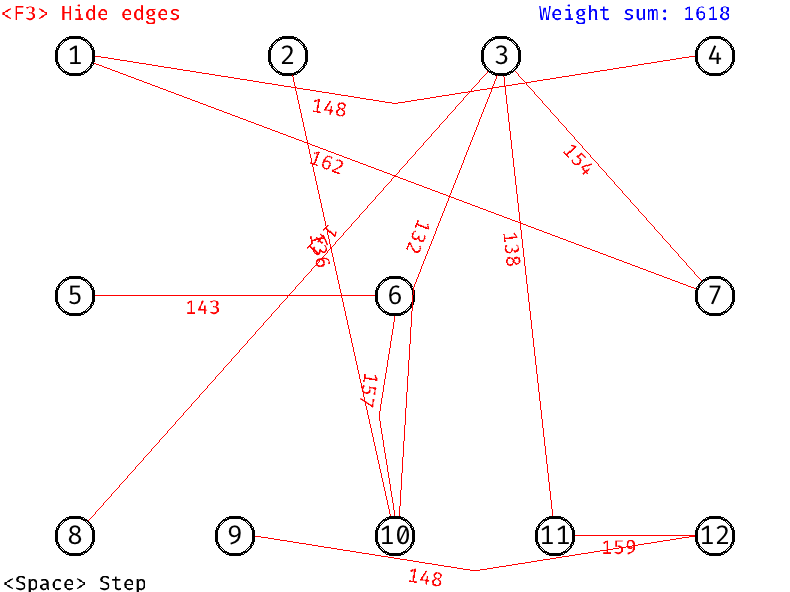
\includegraphics[width=0.5\linewidth]{result.png}
  \caption{Побудований кістяк}
\end{figure}
\pagebreak

\conclusion%
Модифікував представлення графа у програмі для зберігання ваг ребер.\\
Реалізував алгоритм Краскала для покрокової побудови мінімального кістяка ненапрямленого графа.
Використав структуру disjoint set union (так званий\\
\texttt{UnionFind}) для запобігання утворенню циклів.

\end{document}

% vim: ts=2: sw=2
